% !TEX root=/home/tavant/these/manuscript/src/manuscript.tex

\section{Axial convection of the particles}
  \label{sec-reinjectionnoise}

  As introduced in the previous section, the \ac{2D} radial-azimuthal simulation does not model the axial convection of the particles.
  This results in an ever increasing particle energy \citep{lafleur2016a,heron2013}.
  We present in this section an algorithm to model the convection of the particle.
  Its drawbacks are discussed, and we propose a way to reduce them.
  
  \subsection{Lafleur's model of convection}

    \citet{lafleur2016a} proposed a way to model the axial convection of the particles in a \ac{1D} purely azimuthal simulation.
    \Cref{fig-Fake_1d_1} shows a schematic illustration of the model.
    The principle is as follow
    \begin{itemize}
      \item We set a finite axial length, noted $L_z$ in \cref{fig-Fake_1d_1}.
      \item We follow the positions of the particle in the axial direction $z$
      \item When a particle crosses the boundary, it is removed.
      \item A new particle is created
      \begin{itemize}
        \item at $z=0$ for the ions
        \item  at $z=L_z$ for the electrons
      \end{itemize}
    \end{itemize}

    We create a new particle in order to conserve the charge in the simulation.
    The new particle has a velocity following a Maxwellian flux distribution function of a given temperature.
    The azimuthal position of the particle is chosen uniformly at random.

    The Maxwellian flux distribution is the velocity distribution of the particles traversing a surface if the particles follow a Maxwellian distribution function. Thus we have
    \begin{equation} \label{eq-Maxwflux} 
      f_{\rm flux}(\vect{v}) = \vect{v} \cdot \vect{n} f_{\rm M}(\vect{v}),
    \end{equation}
    with $f_{\rm M}$ the Maxwellian distribution function defined in \cref{eq-Maxwellian} and $\vect{n}$ the vector normal to the surface.

    \begin{figure}[hbt]
      \centering
      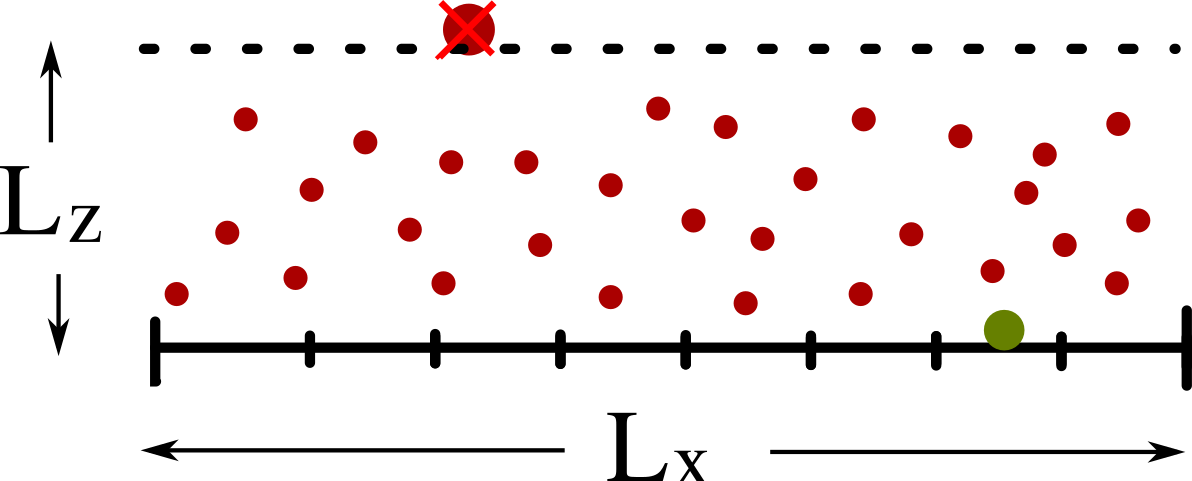
\includegraphics[width=\defaultwidth]{Fake_1d_2}
      \caption{Schematic representation of Lafleur's convection model \citep{lafleur2016a}. The red particle is removed of the simulation, and the green particle is created. In this illustration, the particle is an ion, and the reinjection is at $z=0$. The x direction corresponds to the azimuthal direction.}
      \label{fig-Fake_1d_1}
    \end{figure}

    Lafleur's model of convection has been adopted in \ac{2D} by \citet{croes2017a}.
    The principle is exactly similar.
    The particles are followed in the three directions, and a finite length is used to close the axial direction.
    It is important to note that even if the particles are followed in the three directions, the meshed domain is only \ac{2D}.
    The simulation is not \ac{3D}-\ac{3V}, but only \ac{2D}-\ac{3V}.

    In \citet{croes2017a}, the authors have observed that if the newly created particle has a radial position chosen uniformly at random, it will affect the sheath.
    Hence, they decided to use the same radial position that the removed particle.
    \Cref{fig-Fake_2d} presents a schematic representation of the convection model in \ac{2D}.

    \begin{figure}[hbt]
      \centering
      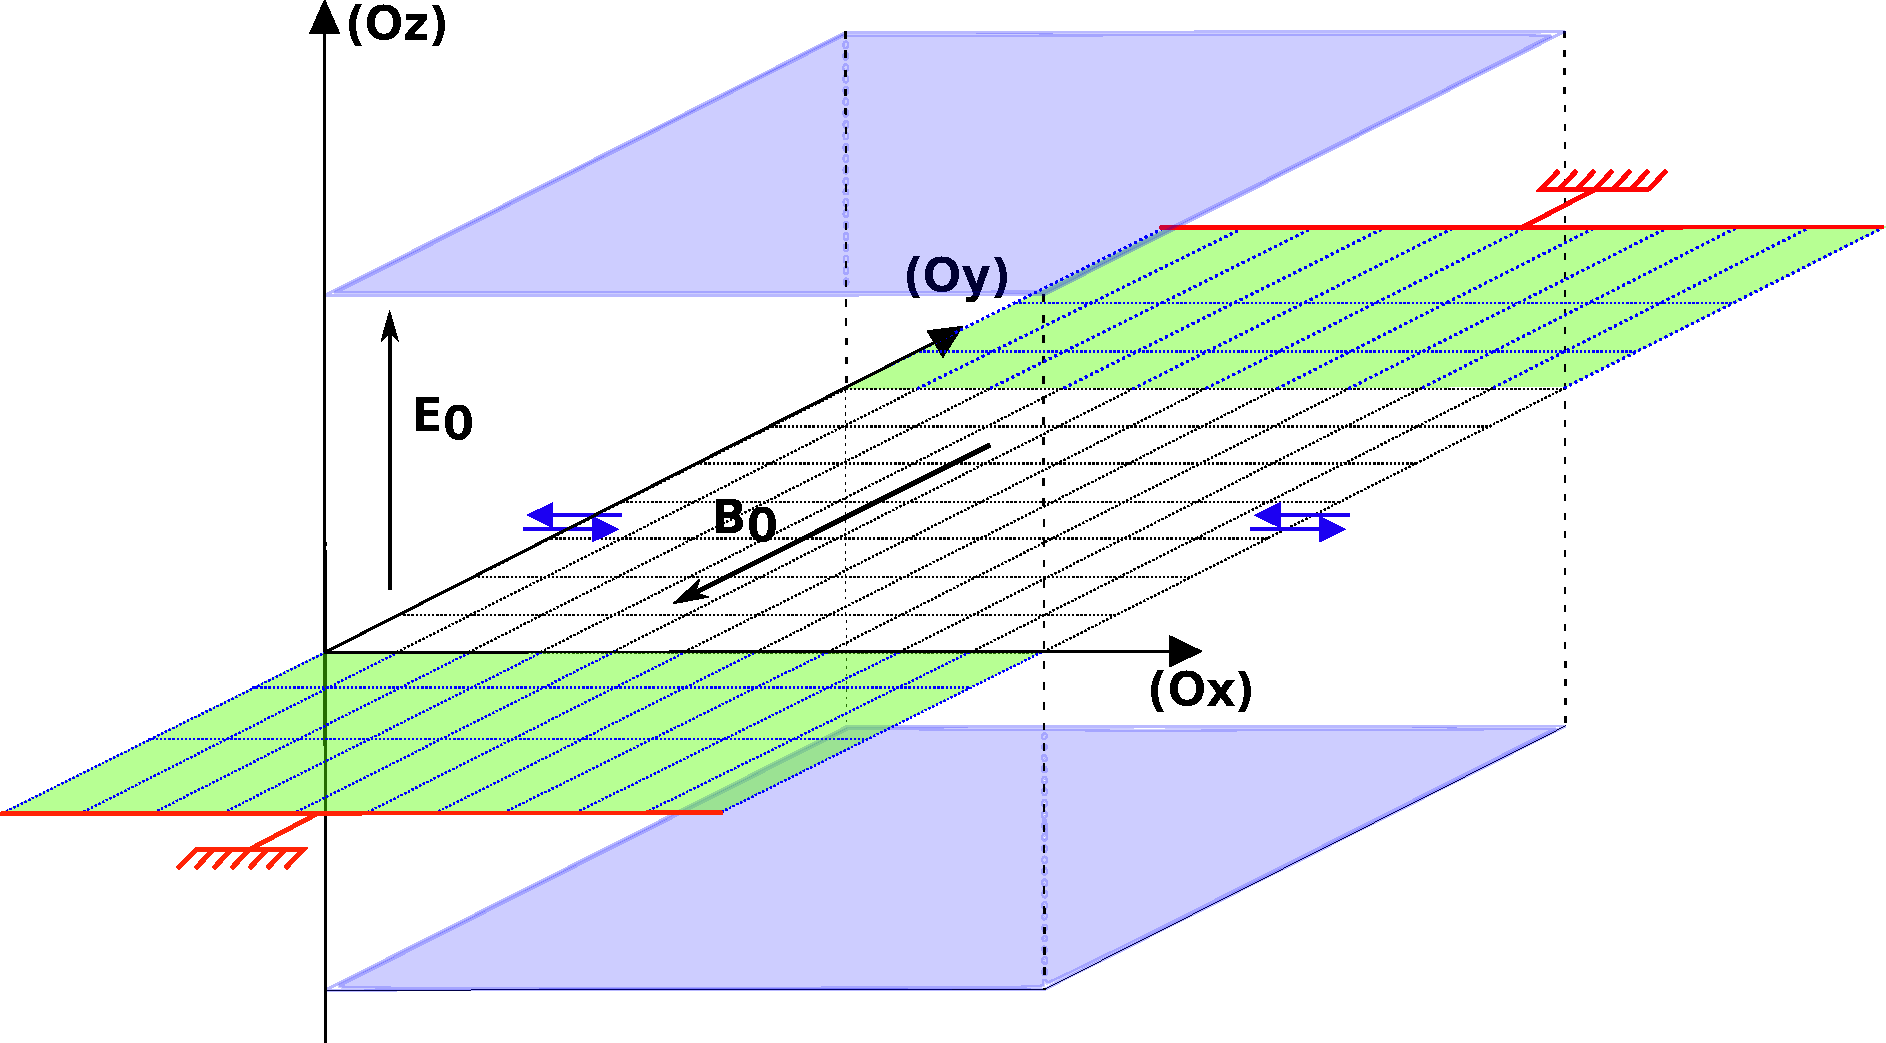
\includegraphics[width=\defaultwidth]{2_5D_dielectric_PPS_small}
      \caption{Schematic representation of the Lafleur's convection model adapted in \acs{2D}. The new particle radial position corresponds to the removed particle, but its azimuthal position is chosen uniformly at random. }
      \label{fig-Fake_2d}
    \end{figure}

    \Cref{fig-energy_convection} shows the evolution as a function of time of the electron mean energy in a typical \ac{2D} radial-azimuthal simulation, adapted from \citet{croes2017}.
    We can see that without the convection, the mean energy quickly rises to unphysical values.
    When the convection is modeled, using an axial of $L_z=1$ cm, the energy reaches a steady-state.
    \nomenclature[Q]{\ensuremath{ L_z}}{ Axial length}
    \begin{figure}[hbt]
      \centering
      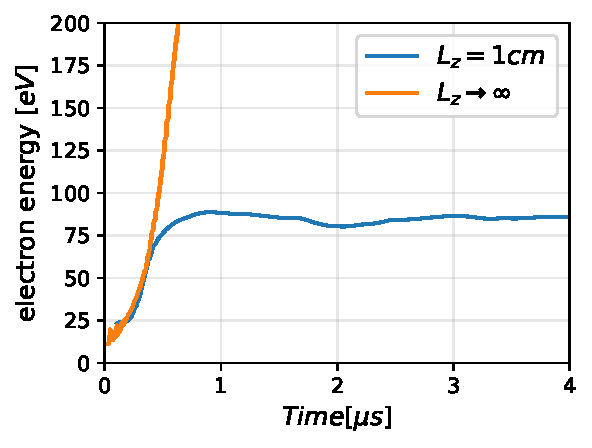
\includegraphics[width=\defaultwidth]{energy}
      \caption{Time evolution of the electron mean energy when the convection is not modeled ($L_z \rightarrow \infty$) and with Lafleur's convection model used, $L_z = 1$ cm. Adapted from \citet{croes2017}.}
      \label{fig-energy_convection}
    \end{figure}



  \subsection{Numerical artifacts}
    \citet{lafleur2016a} studied the impact of the convection model on the simulation results.
    The authors observed in particular that changing the azimuthal length of the simulation domain could affect the simulation results.

    \Cref{fig-convection_numerical} shows the time evolution of the azimuthal electric field $E_{\theta}$ from the \ac{1D} simulation \citep{lafleur2016a}.
    \nomenclature[Q]{\ensuremath{ E_{\theta}}}{ Azimuthal electric field}

    On the first row (\cref{fig-convection_numerical}.{\bf a} and {\bf b}), the length of the periodic azimuthal direction is $L_{\theta}=0.5$~cm.
    \cref{fig-convection_numerical}.{\bf a} corresponds to the case without axial convection.
    We see that the \ac{ECDI} rises and does not saturate.
    The wavelength is short, of the order of $\lambda = 1.5$~mm.
    \nomenclature[Q]{\ensuremath{ \lambda}}{ Wave length}
    \cref{fig-convection_numerical}.{\bf b} corresponds to the same case as \cref{fig-convection_numerical}.{\bf a} but this time with the axial convection modeled.
    We observe this time a saturation of the oscillation's amplitude, and the wavelength is close to $\lambda \simeq 1.5$~mm.

    On the second row (\cref{fig-convection_numerical}.{\bf c} and {\bf d}), the length of the periodic azimuthal direction is $L_{\theta}=1$~cm.
    \cref{fig-convection_numerical}.{\bf c} corresponds to the case without axial convection, and \cref{fig-convection_numerical}.{\bf d} corresponds to the same case but with the axial convection modeled.
    In \cref{fig-convection_numerical}.{\bf c}, we can see that increasing the azimuthal length compared to \cref{fig-convection_numerical}.{\bf a} did not affect the \ac{ECDI}, as expected.
    However, in  \cref{fig-convection_numerical}.{\bf d}, the instability is clearly affected.
    A single oscillation is observed, corresponding to $\lambda=10$~mm, which seems almost undoubtedly unphysical.

    \begin{figure}[hbt]
      \centering

      \begin{tabular}{@{} cc @{}}
        \subfigure{Lafleur_NoLz_1}{a}{20, 20}  &
        \subfigure{Lafleur_Lz_1}{b}{20, 20} \\
        \subfigure{Lafleur_NoLz_2}{c}{20, 20} &
        \subfigure{Lafleur_Lz_2}{d}{20, 20} \\
      \end{tabular}
      \caption{Effects of Lafleur's convection model for two different azimuthal lengths on the azimuthal electric field. ({\bf a}) No convection, $L_x=0.5$~cm,  ({\bf b}) convection modeled, $L_x=0.5$~cm,  ({\bf c}) No convection, $L_x=1$~cm,  ({\bf d}) convection modeled, $L_x=1$~cm. The color of each plot is normalized to the maximum amplitude. Adapted from \citep{lafleur2016a}. }
      \label{fig-convection_numerical}
    \end{figure}
    \FloatBarrier
    \citet{croes2017} observed similar behavior with the bidimensional  simulation.
    The author investigated the values of the azimuthal length, which presented physical and unphysical results
    for different values of the axial length.
    \Cref{fig-couplesCroes} shows the results obtained (adapted from \citep{croes2017}).
    We can see that for a given value of the axial length, the azimuthal length must be less than a specific value to present physical results.
    However, the value of this upper limit depends on the axial length, such that if the axial length decreases, the upper limit of the azimuthal length decreases as well.

    \begin{figure}[hbt]
      \centering
      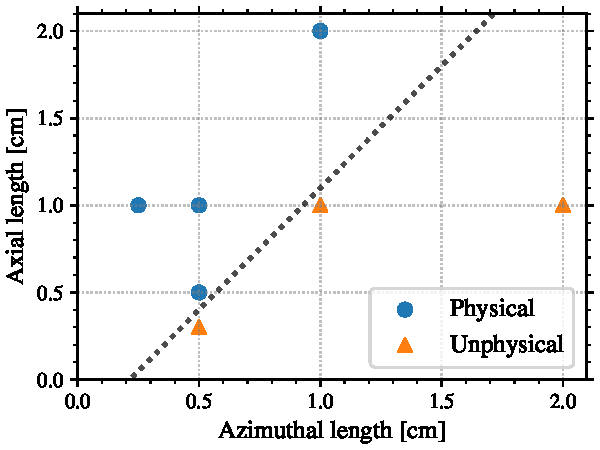
\includegraphics[width=\defaultwidth]{2D_couples.pdf}
      \caption{For 2D PIC simulations\string: values of the azimuthal length and the axial length for which the simulation result is physical (similar to \cref{fig-convection_numerical}.{\bf b}) or unphysical  (similar to \cref{fig-convection_numerical}.{\bf d})}
      \label{fig-couplesCroes}
    \end{figure}

    In the next section, we develop a theory that could explain the observation, and a new convection model for the simulation is proposed.

  \subsection{Numerical noise of Lafleur's convection model}

    Let us consider Lafleur's convection model in \ac{1D} on the charge density.
    When computing the charge density on the mesh vertices, the axial position is not taken into account.
    Consequently, the convection process illustrated in \cref{fig-Fake_1d_1} is similar to moving a particle arbitrarily (read randomly).
    Seen by the charge density, this is similar to Poisson noise, also named shot noise, on the charge density.\footnote{Actually, this noise is the combination of Poisson noise with a uniform noise, happening twice for every particle convection, once with a positive charge and once with a negative charge.}

    After a certain number of particles removed and created, the Poisson noise is similar to a Gaussian noise, also named thermal noise, following a normal distribution $\N$. 
    \nomenclature[Q]{\ensuremath{ \N }}{ Normal distribution.}
    Hence, the charge density becomes \footnote{One can note that the mean of the noise is strictly zero (with probability 1), as the charge density is conserved.}
    \begin{equation} \label{eq-rhonoise}
      \rho = \rho_0 + \N(0, \stdconv),
    \end{equation}
    with $\rho$ the charge density, $\rho_0$ the charge density without the convection process, and $\stdconv$ the standard deviation of the distribution of the noise associated with the convection model.
    \nomenclature[Q]{\ensuremath{ \rho}}{ Charge density}
    \nomenclature[Q]{\ensuremath{ \stdconv}}{ tandard deviation of the distribution of the noise associated with the convection model}
    Surprisingly, the noise due to the convection model is similar to the numerical noise induced by the decomposition of the plasma into particles $\N(0, \sigma_{\rm stat})$.
    However, the amplitude of this statistical noise decreases with the number of particles per cell used
    \begin{equation*} \label{eq-statistical}
     \sigma_{\rm stat} \propto \frac{1}{\sqrt{N_{pc}}}.
    \end{equation*}

    On the other hand, the amplitude of the noise induced by the convection model depends on the plasma density $n$, the axis velocity of the particles $v_z$ and the axial length $L_z$
    \begin{equation} \label{eq-convstd}
     \stdconv \propto \frac{n}{L_z} v_z.
    \end{equation}

    We can see in \cref{eq-convstd} that the amplitude of the convection induced noise on the charge density is proportional to the inverse of the axial length $L_z$.
    This could explain the observation of \cref{fig-couplesCroes} when using a smaller $L_z$.
    However, it does not explain the effects of the azimuthal length observed in \cref{fig-couplesCroes,fig-convection_numerical}.

  \subsection{Effect of the noise on the electric field}
    \label{sec-mathnoise}
    In order to explain the impact of the azimuthal length on the instability, we can study the azimuthal electric field $\aziE$ resulting of the charge density $\rho$.
    As the Poisson equation is linear, we have
    \begin{align}
      \aziE(\theta) &= C + \frac{1}{\epsilon_0} \int_0^{\theta} \rho(s) ds\\
                    &= C + \frac{1}{\epsilon_0} \int_0^{\theta} (\rho_0(s) + \N(0, \stdconv) ) ds \\ 
                    &= C + \aziE_{, 0} + \aziE_{, 1}
    \end{align}
    with $C$ a constant that ensures that the periodical \ac{BC} are respected.
    The part of the electric field $\aziE_{, 0}$ corresponds to the unperturbed charge density $\rho_0$ and $\aziE_{, 1}$  corresponds to the noisy charge density $\N(0, \sigma_{\rm stat})$.
    Hence, let us focus now on $\aziE_{, 1}$.
    We can study $\aziE_{, 1}$ using two equivalent means\string: the \ac{FT} and the Brownian bridge.
    
    \paragraph{Fourier Transform \\}
      Applying the \ac{FT} on the equation
      \begin{equation} \label{eq-aziE1}
        \aziE_{, 1} = \frac{1}{\epsilon_0} \int_0^{\theta}  \N(0, \stdconv) ds
      \end{equation}
      gives    
      \begin{align}
        \FFT \lp \aziE_{, 1} \rp (k) &= \frac{1}{\epsilon_0} \FFT \lp \int_0^{\theta}  \N(0, \stdconv) ds \rp \\
                                     &= \frac{1}{\epsilon_0} \frac{ \N(\mu_{\rm FT}, \sigma_{\rm FT})}{k} \label{eq-fft}
      \end{align}
      
      \Cref{eq-fft} shows that $\aziE_{, 1}$ also follows a Gaussian distribution, but with a non-zero mean value.
      It is also inversely proportional to the wave number $k$.
      Hence, when we increase the azimuthal length, which means that small wave numbers can exist in the simulation domain, the amplitude of $\aziE_{, 1}$ increases as well.
      
    \paragraph{Brownian Bridge\\}
      \Cref{eq-aziE1}, combined with the \ac{BC}, is the definition of the a Brownian bridge.
      
      A Brownian bridge is a particular Brownian motion that reaches at a given distance the same value as the initial value.
      Hence, we have \citep{ibe2013}
      \begin{align*}
        \mathbb{E}(\aziE_{, 1}) &= 0,  \\
        {\rm var}(\aziE_{, 1}) &= \stdconv^2 \frac{L_{\theta^2}}{4}
      \end{align*}
    
      Hence, the increase of the azimuthal length increases the amplitude of $\aziE_{, 1}$.
      
    
    We believe that when the amplitude of $\aziE_{, 1}$ is too large, it can trigger an unphysical oscillation.
    The next section uses this conclusion in order to adapt the convection model.
    
    \subsection{Noiseless convection model}
      \label{sec-noiselessresults}
      In previous section, we have shown that the convection model induces a noise in the charge density, that produces an azimuthal electric field which amplitudes depends on the azimuthal length.
      
      We propose here a modified version of Lafleur's convection model in order to remove the noise in the charge density.
      The noiseless convection model follows the same algorithm as before, but the azimuthal position of the particle created is not chosen uniformly as random, but instead the new particle has the same position as the removed particle.
      \Cref{fig-fakez3} shows a schematic illustration of the noiseless convection algorithm applied on a particle.
      
      \begin{figure}[hbt]
        \centering
        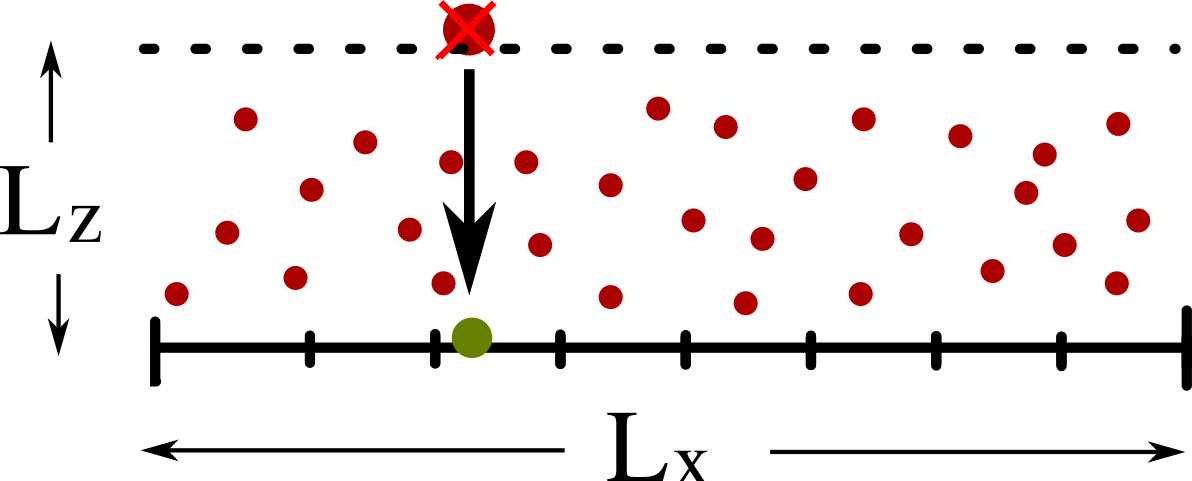
\includegraphics[width=\defaultwidth]{Fake_1d_3}
        \caption{Illustration of the noiseless convection model}
        \label{fig-fakez3}
      \end{figure}
      
      We have implemented this modified convection model in the \ac{2D} radial and azimuthal simulation.
      \Cref{fig-newconv_noconv} shows the time  evolution of the azimuthal electric field at the center of the radial dimension with and without the noiseless convection model.
      It presents the same conditions as in \cref{fig-convection_numerical}.{\bf a} and {\bf b}. 
      As previously, the convection stabilizes the growth of the instability to a steady-state, but it does not affect the physics.
       
      
      \begin{figure}[hbt]
        \centering
        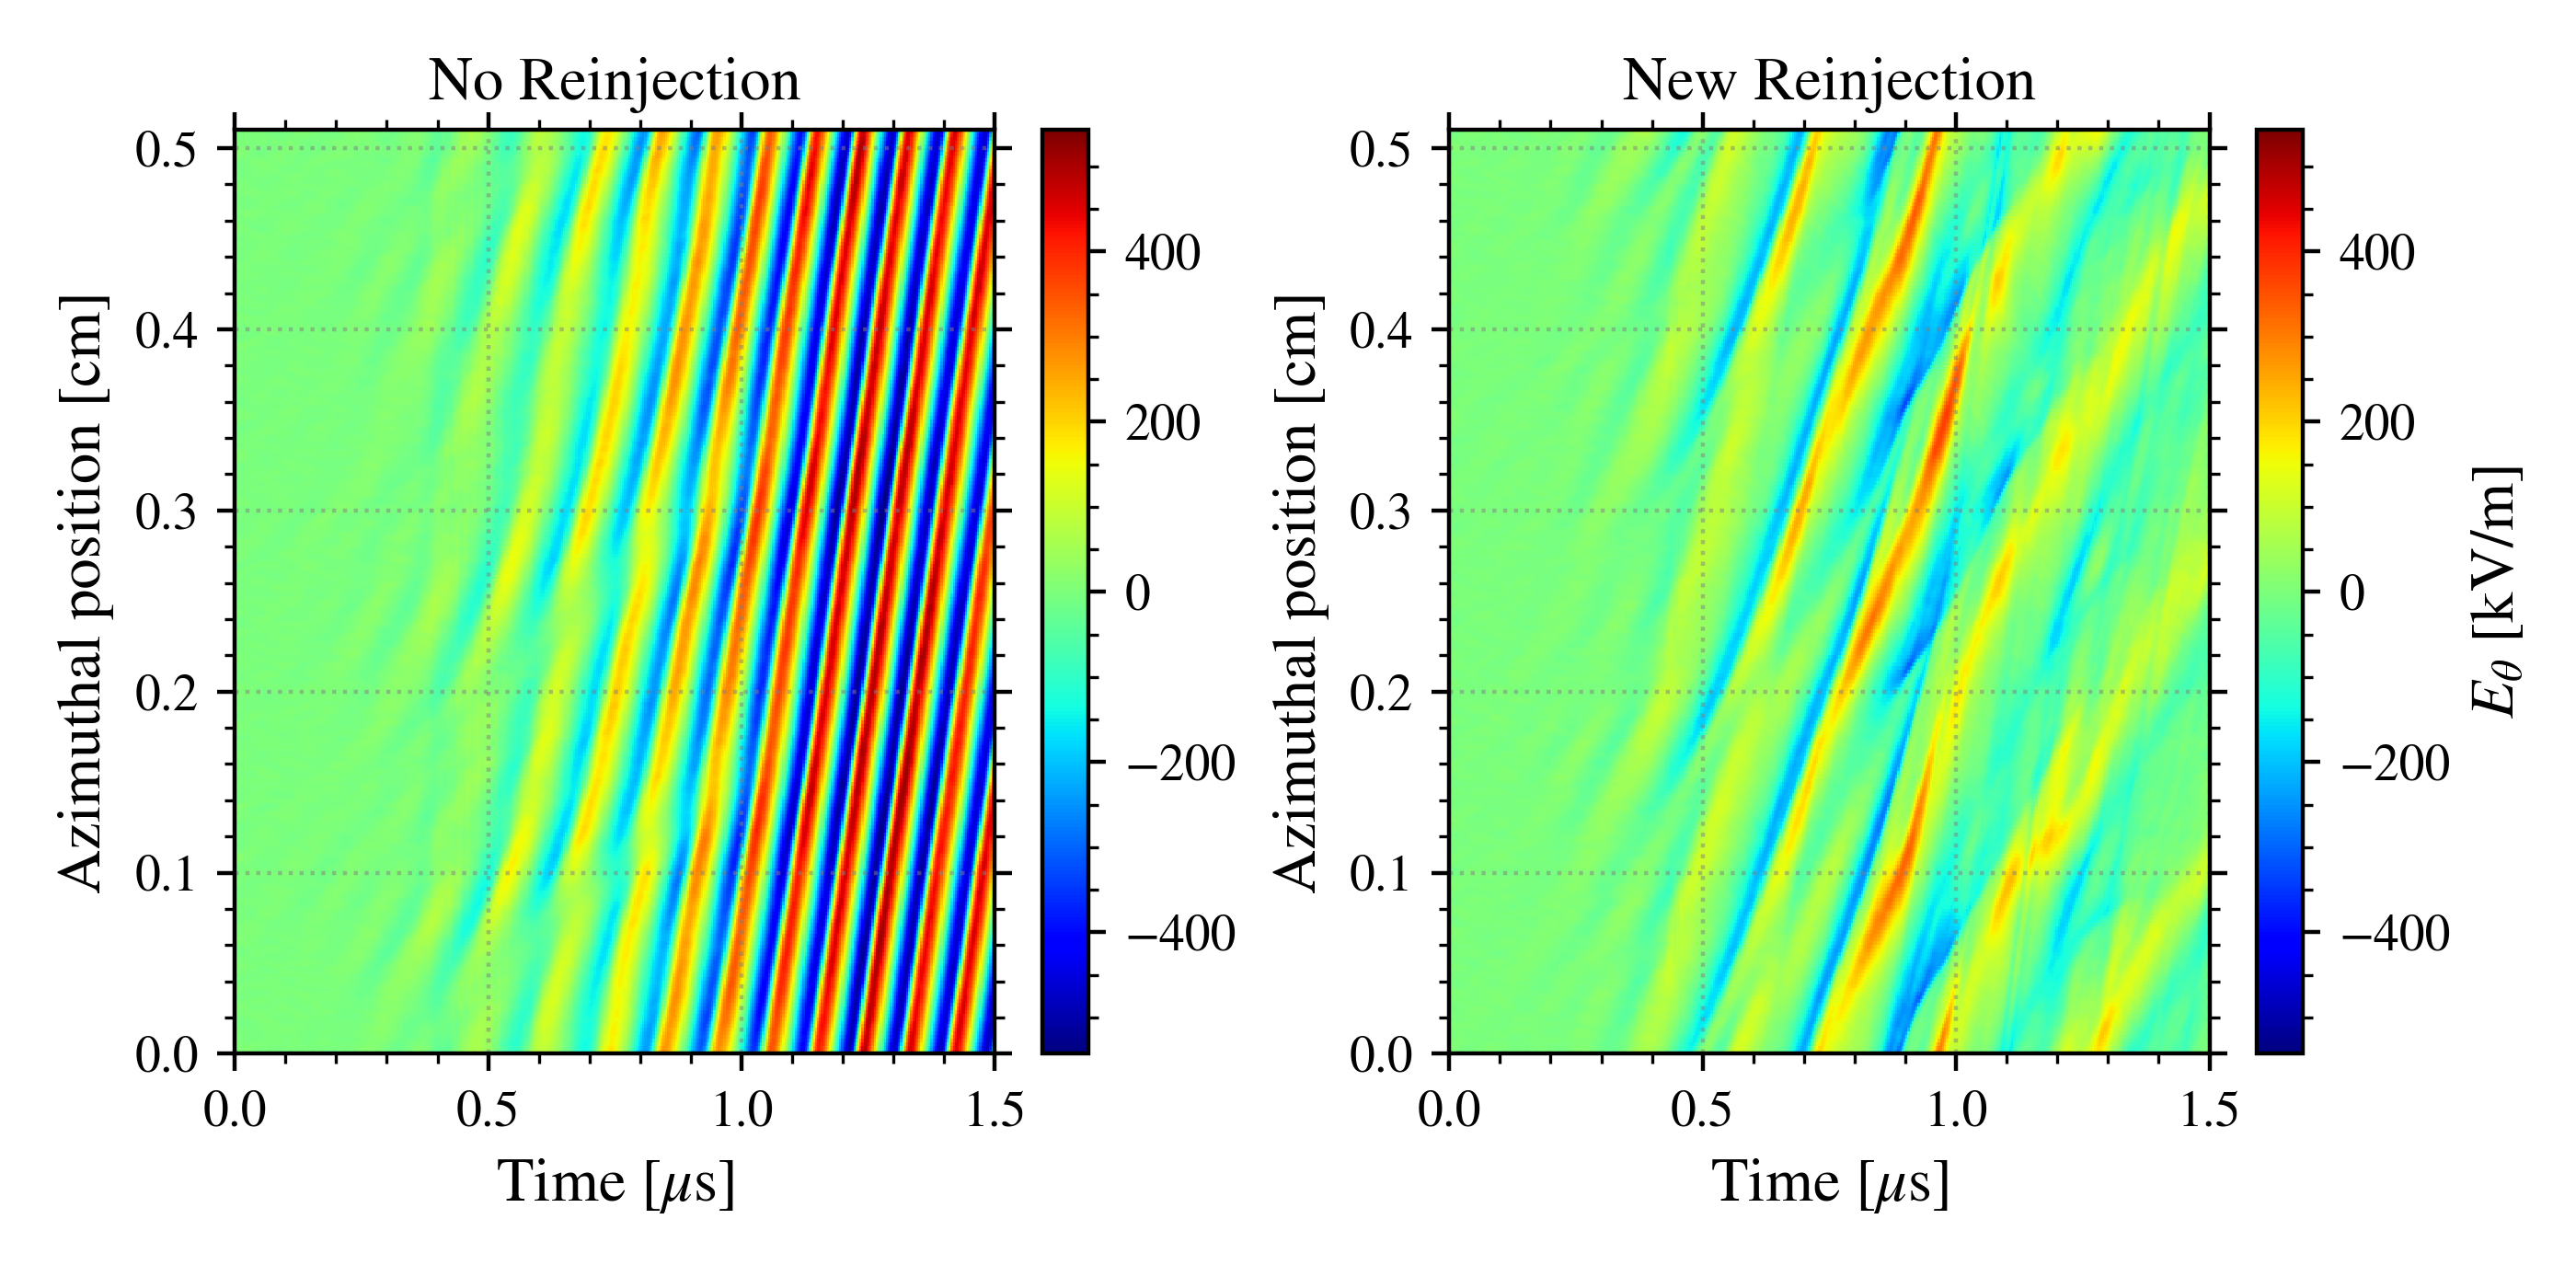
\includegraphics[width=0.95\textwidth]{Compare_no_new_Reinj_Oz}
        \caption{Time evolution of the azimuthal electric field at the center of the radial dimension with and without the noiseless convection model. }
        \label{fig-newconv_noconv}
      \end{figure}
      
      
      \Cref{fig-oldeconv_newconv} shows the time  evolution of the azimuthal electric field at the center of the radial dimension  with the convection modeled using Lafleur's model and the noiseless model with a small azimuthal length.
      We can see that the two models give almost exactly the same results.
      
      \begin{figure}[hbt]
        \centering
        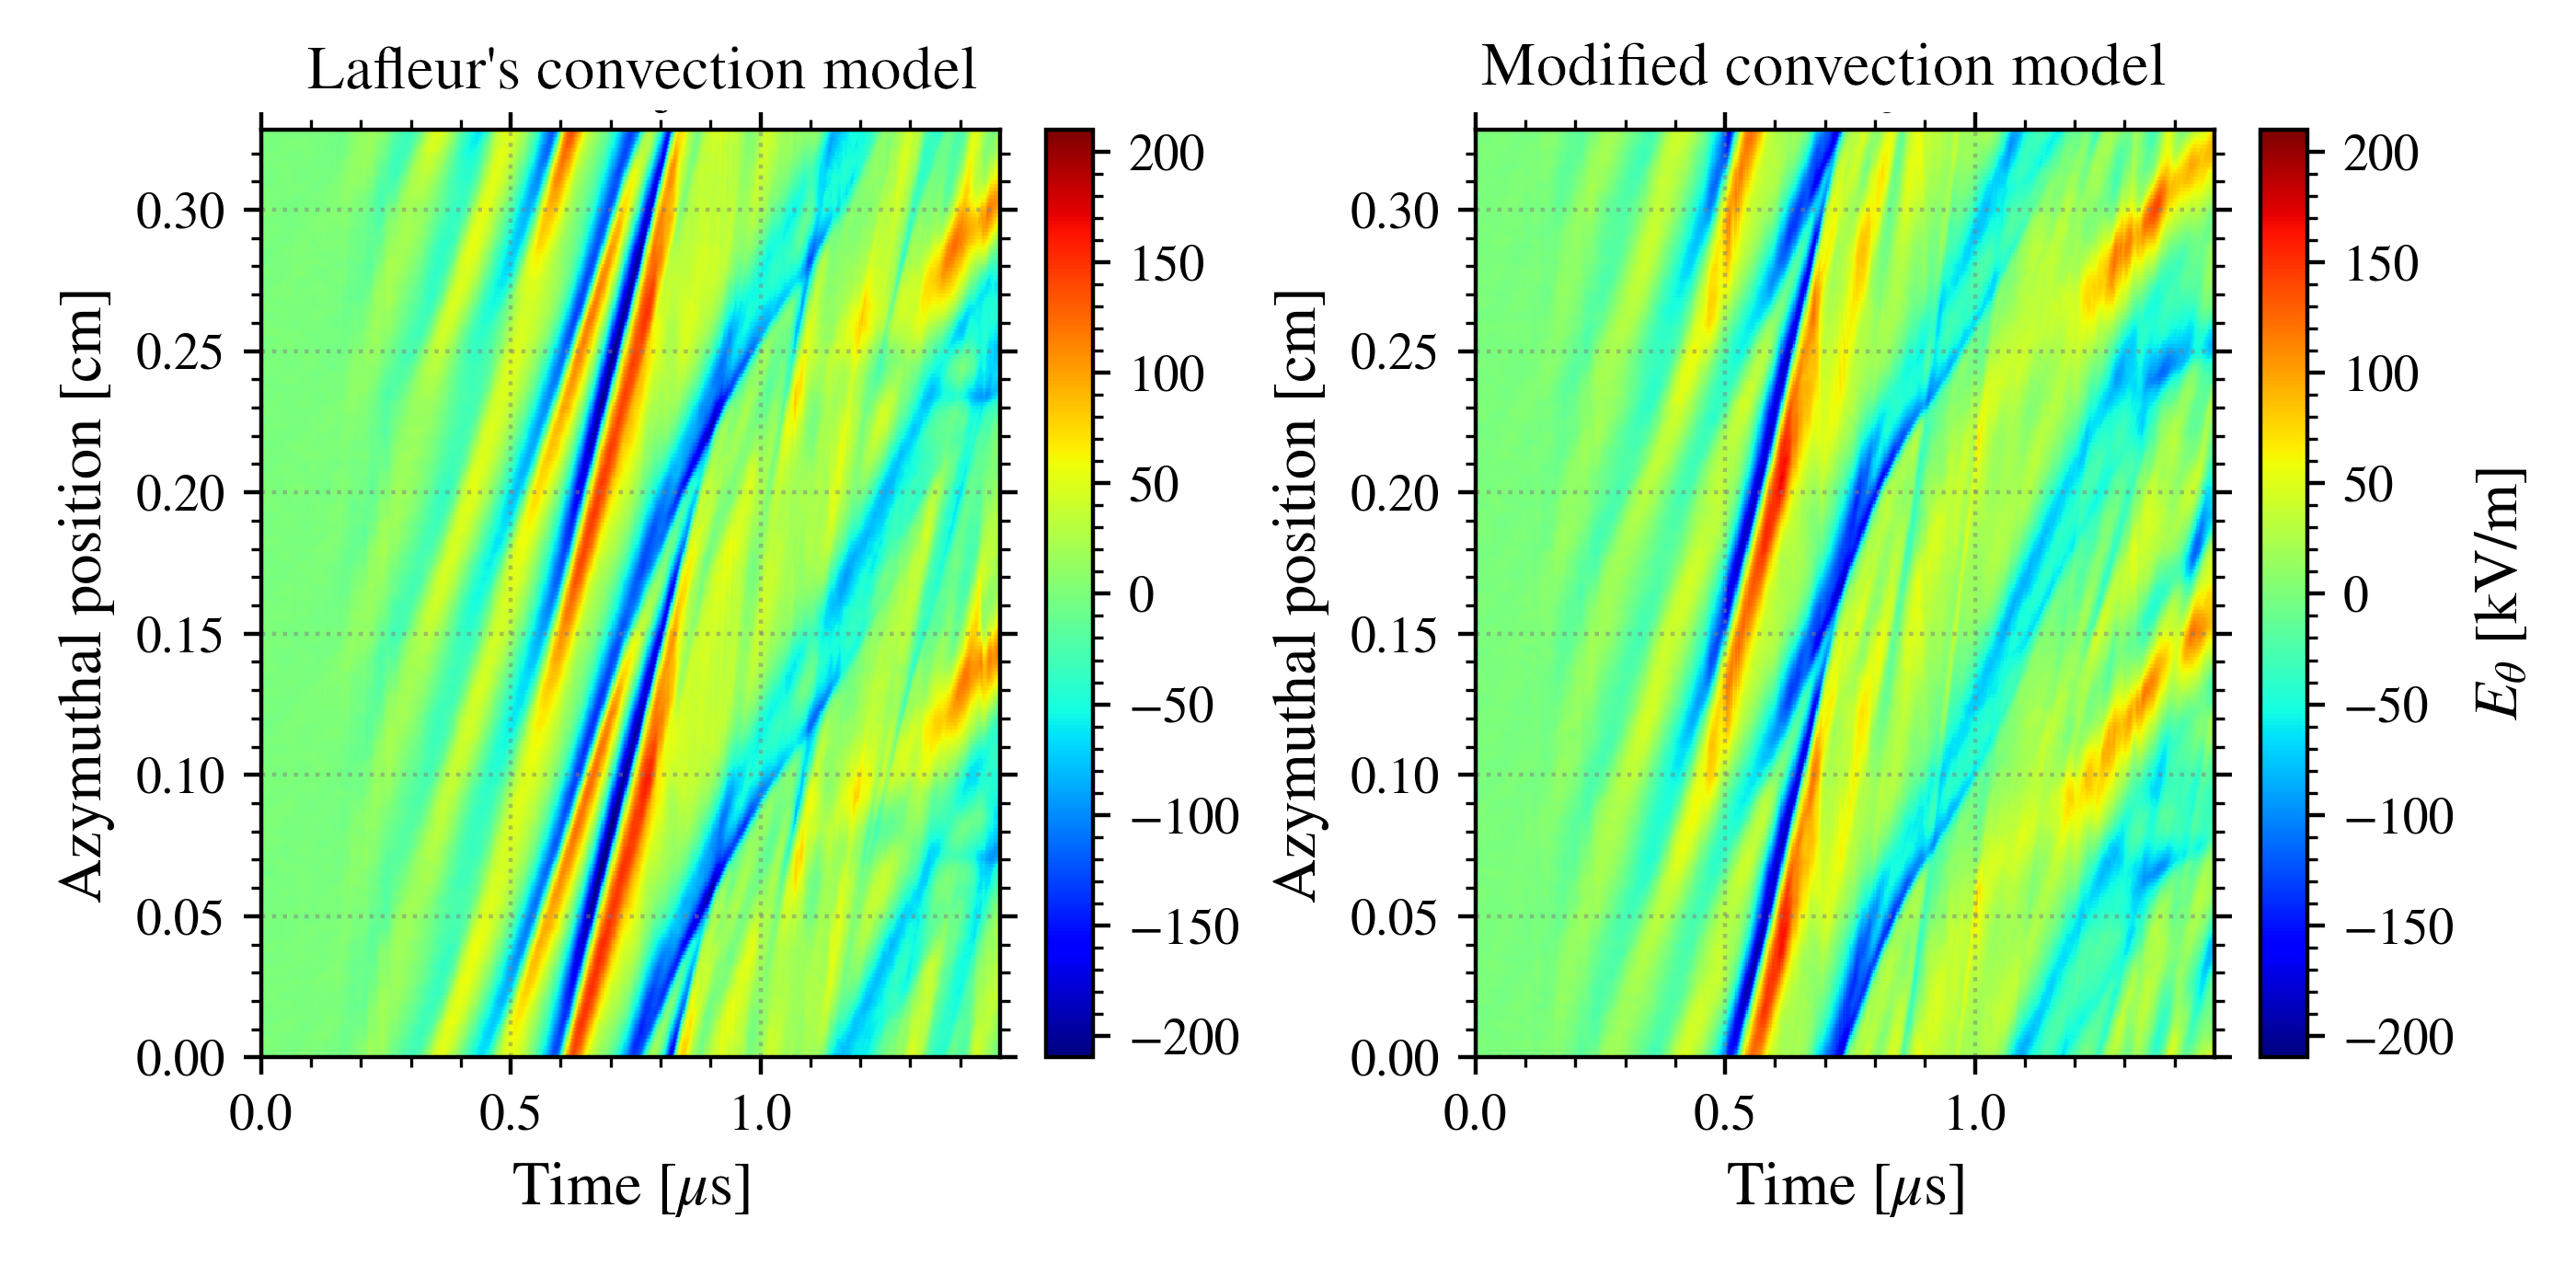
\includegraphics[width=0.95\textwidth]{Compare_old_new_Reinj_Oz}
        \caption{Time evolution of the azimuthal electric field at the center of the radial dimension with the convection modeled using (left) Lafleur's model and (right) the noiseless model with a small azimuthal length (0.325cm).}
        \label{fig-oldeconv_newconv}
      \end{figure}
      
      
      \Cref{fig-oldeconv_newconv_longLZ} shows the  time  evolution of the azimuthal electric field at the center of the radial dimension  with the convection modeled using Lafleur's model and the noiseless model but using a longer azimuthal length than \cref{fig-oldeconv_newconv}.
      In this case, we can see that Lafleur's convection model induces oscillations that are not observed with the noiseless model.
      
      \begin{figure}[hbt]
        \centering
        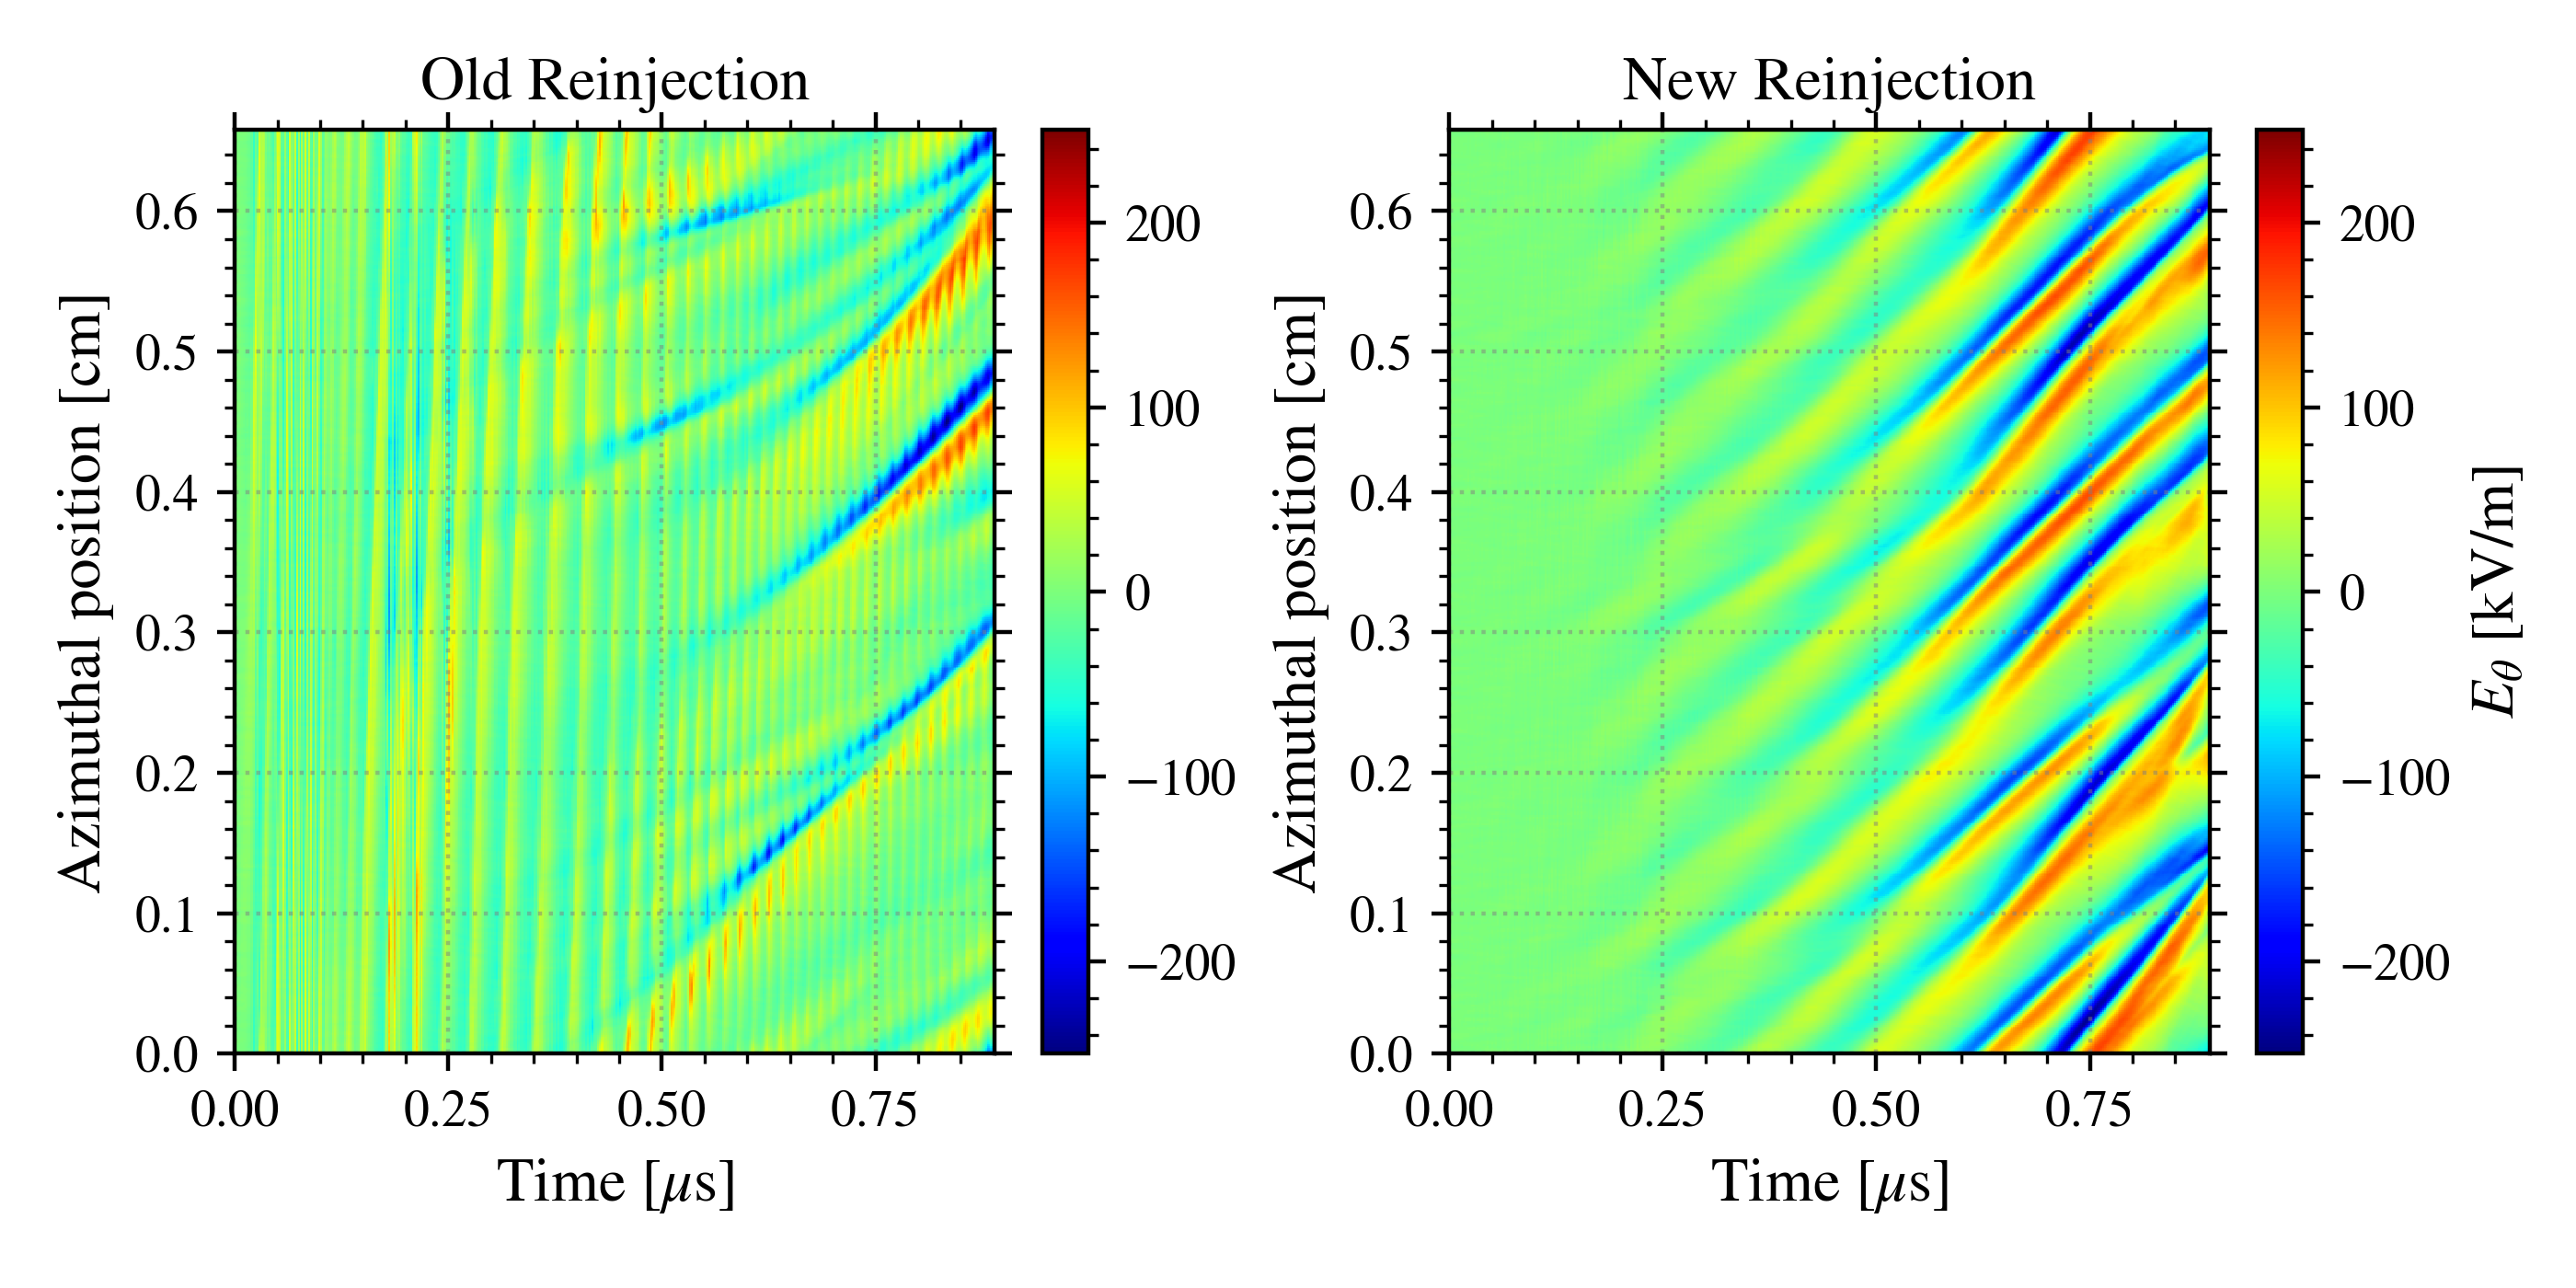
\includegraphics[width=0.95\textwidth]{Compare_old_new_Reinj_Oz_LongLx}
        \caption{Time evolution of the azimuthal electric field at the center of the radial dimension with the convection modeled using (left) Lafleur's model and (right) the noiseless model with a longer azimuthal length (0.65cm).}
        \label{fig-oldeconv_newconv_longLZ}
      \end{figure}


      These observations have shown that Lafleur's convection model induces a noise on the charge density, that does not affect the simulation when the domain size is small, but can rise numerical artifacts when the domain size is larger.
      We have seen that the minor modifications on the model do not affect the simulation results on a small domain, and allows us to use a larger simulation domain without any numerical artifact.
      
      
          
    \subsection{Effects on a \acs{2D} simulation domain}
      
      The mathematical development of \cref{sec-mathnoise} has been done in \ac{1D}.
      We can legitimately wonder if the results  can be extended directly to a \ac{2D} domain.
      A mathematical definition of $\aziE_{, 1}$ i \ac{2D} is more difficult, as we have, neglecting the dielectric layers,
      \begin{equation} \label{eq-aziE}
        \aziE_{, 1} = -\partial_{\theta} \phi_1 \text{ such that } \grad \cdot \grad \phi_1 = - \frac { \N(0, \stdconv)}{\epsilon_0} \text{ following the \ac{BC}}.
      \end{equation}
      The \ac{BC}s are
      \begin{itemize}
        \item periodic \ac{BC} in the azimuthal direction,
        \item Dirichlet \ac{BC} in the radial direction, modeling grounded walls,
      \end{itemize}
      which translate as
      \begin{align}
        &\phi = 0 \text{ for } r=0 \text{ and } r=L_r, &\forall \theta \label{eq-BC1} \\
        &\phi(\theta = 0)= \phi(\theta = L_{\theta}) , &\forall r \label{eq-BC2}
      \end{align}
      
      Solving \cref{eq-aziE} with the conditions \cref{eq-BC1,eq-BC2} analytically is much more difficult that the \ac{1D} development, because of the Dirichlet \ac{BC}.
      \nomenclature[N]{Dirichlet Boundary condition\string:}{ a type of boundary conditions for which the field is fixed. For instance for grounded electrodes on the plasma potential\string: $\phi = 0$}
      However, we can investigate it numerically, by solving \cref{eq-aziE} for a given random source term.
      Using a Monte Carlo approach, we average the results  200 times to better observe the mean behavior in respect to the noise (i.e. increasing signal to noise ratio).
      For each computation, a normalized source term $\rho_1 = \N(0, 1)$ is generated over a \ac{2D} domain, then the \ac{2D} Poisson equation is solved numerically\footnote{The SOR algorithm is used in this MC calculation. The iterations are stopped using a relative tolerance of $\sn{2}{-6}$ on the mean square error.} to obtain $\phi_1$, and the azimuthal electric field $\aziE_{, 1} =- \partial_{\theta} \phi_1 $ is computed.
    
      \begin{figure}[hbt]
        \centering
        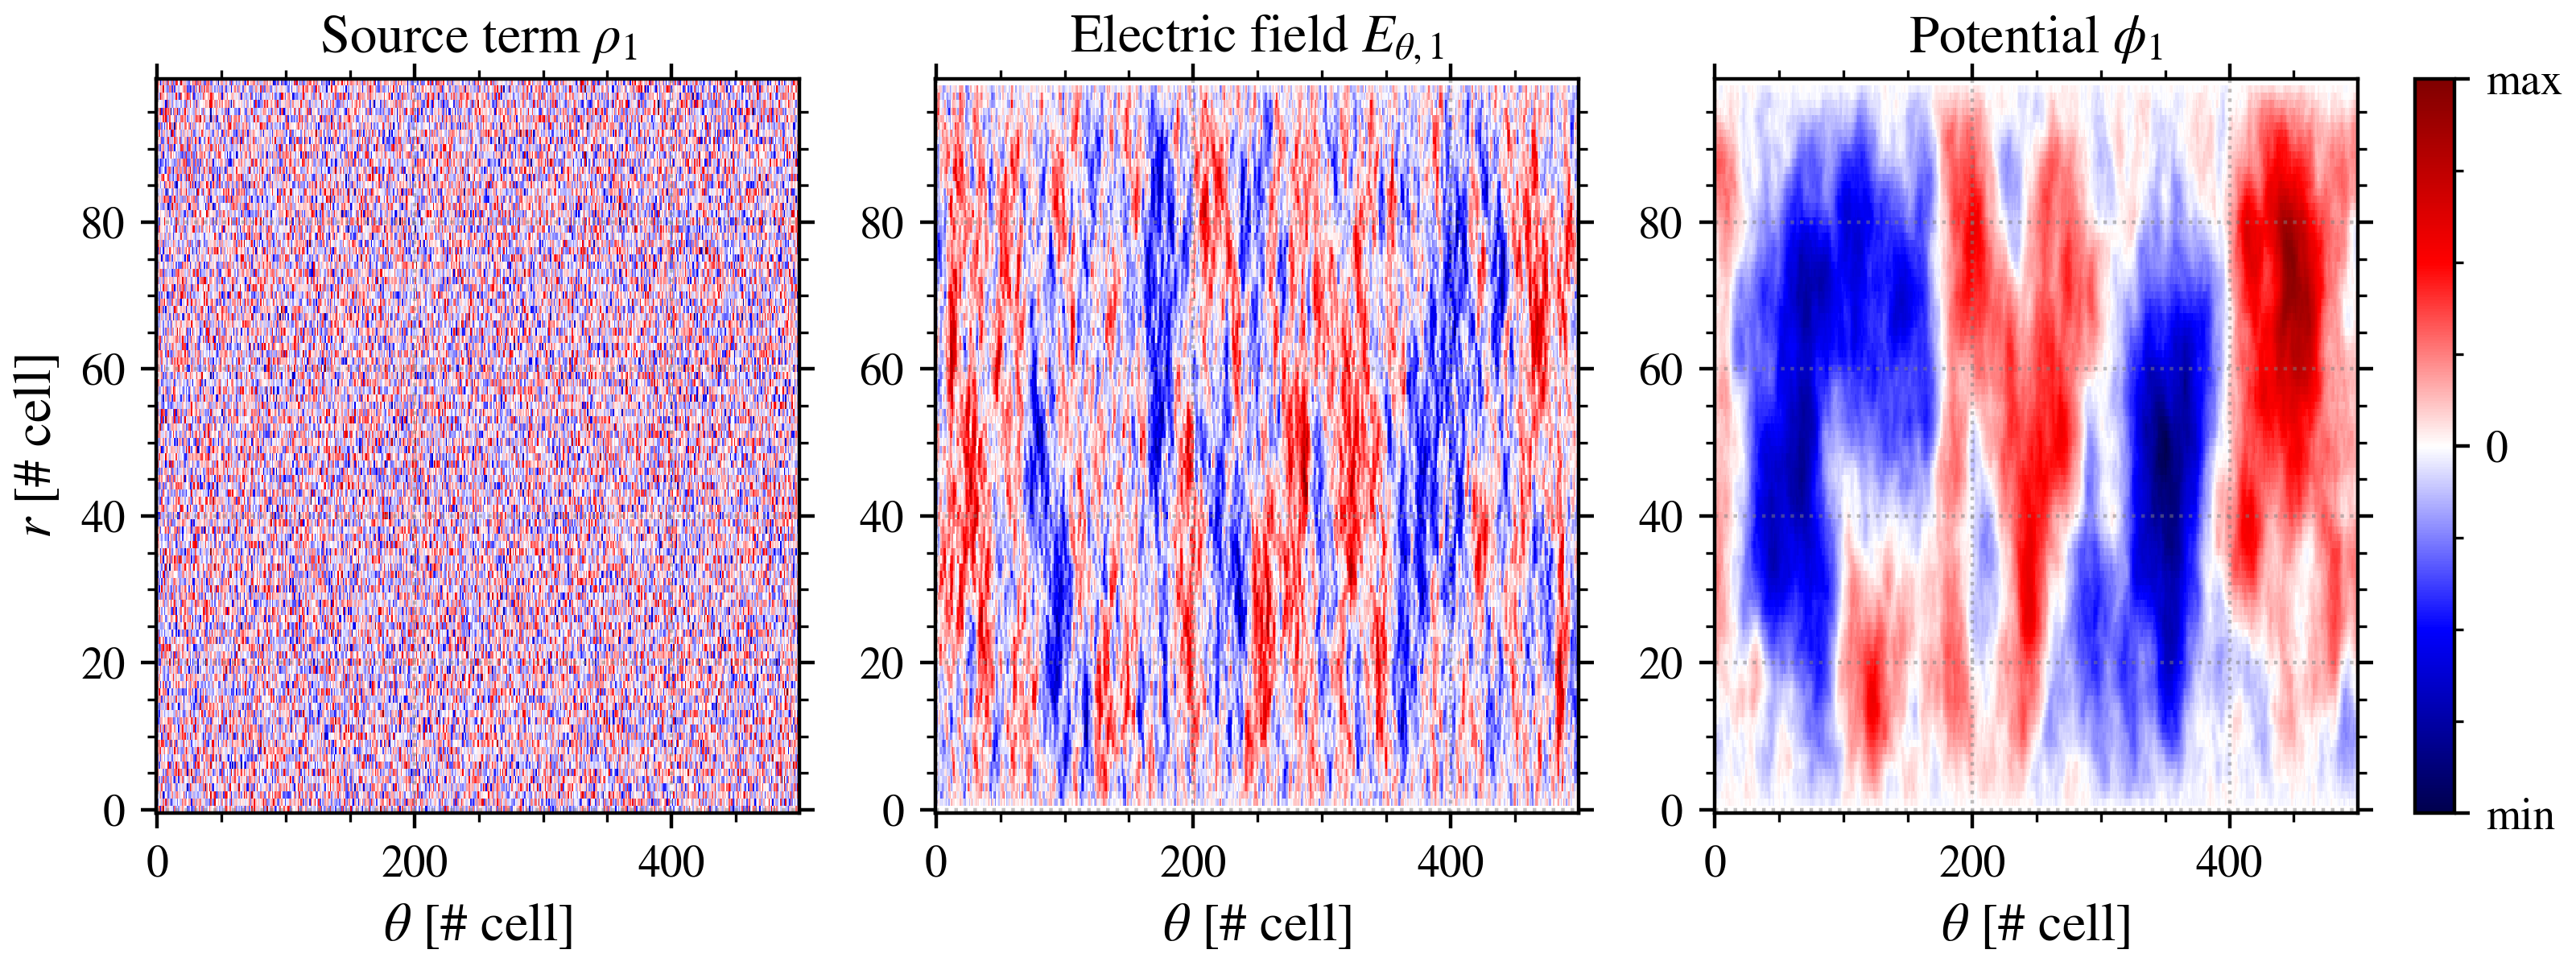
\includegraphics[width=\textwidth]{2D_MC_noise.png}
        \caption{Results for one case used in the Monte Carlo calculation with 100 cells in radial direction and 500 cells in the azimuthal direction, with (left) the normalized source term $\rho = \N(0, 1)$, (center) the azimuthal electric field, and (right) the plasma potential. }
        \label{fig-one}
      \end{figure}
      
      One typical result is shown in \cref{fig-one}.
      We can see the impact of the radial Dirichlet boundary conditions, \cref{eq-BC1}, on the potential $\phi_1$ induced by the noise.
      The potential mostly oscillates in the azimuthal direction, and its amplitude is larger on the centerline between the walls.
      A similar behavior is observed for the azimuthal electric field.      
      
      \Cref{fig-dftLr} shows the \ac{DFT} of the source term $\rho_1$, the resulting azimuthal electric field $\aziE_{, 1}$ and plasma potential $\phi_1$ computed on the centerline of the simulation domain, for three different radial lengths expressed in number of cells in the radial direction $N_x$.
      Is also shown the "equivalent" source term $\rho_{\rm eq}$, which is the source term that would give the frequency spectra of $\aziE_{, 1}$ observed in a \ac{1D} domain
      
      \begin{equation} \label{eq-equirho}
        \rho_{\rm eq} = \epsilon_0 \partial_\theta \aziE_{, 1}.
      \end{equation}
      The results are given for different radial lengths $N_x=15,50 \text{ and } 200$, while the azimuthal length $N_y=200$ is kept constant.
      We can see that the plasma potential and the electric field show larger amplitudes for small wave numbers (large wavelength) compared to large wave numbers in the three cases.
      However, the amplitude of the smallest wave numbers is affected.
      In the cases of small radial length ($N_x=15 \text{ and } 50$), the spectra of the electric field is not monotonic.
      This can be explained by the Dirichlet \ac{BC}s that {\it pins down} the fluctuation of the plasma potential.
      
      To compare the results to the purely azimuthal \ac{1D} case, \cref{fig-dftLr} shows the frequency spectra of the equivalent source term $\rho_{\rm eq}$.
      We see that $\rho_{\rm eq}$ is always smaller than $\rho_1$, and is significantly reduced in the small and large wavenumber.
      However, even though the amplitude is reduced in \ac{2D} with small radial direction compared to a \ac{1D} model, we still observe large amplitude of small wave number oscillations in both the electric field and the plasma potential.
      It means that the \ac{2D} domain does not change significantly the effect of the numerical noise $\rho_1$.
      Hence, the conclusions of  \cref{sec-mathnoise} derived in \ac{1D} can be legitimately used for \ac{2D} domains.
      
      \begin{figure}[hbt]
        \centering
        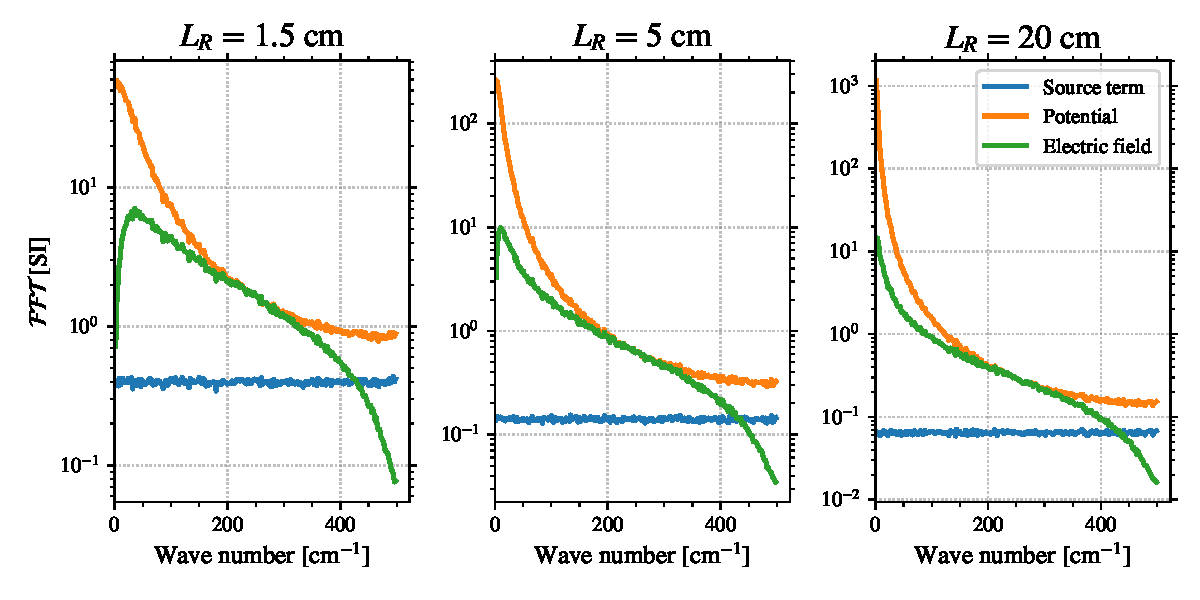
\includegraphics[width=\textwidth]{effect_Lr_noEq1D.pdf}
        \caption{ DFT of the source term $\rho_1 = \N(0, \stdconv)$, the resulting azimuthal electric field $\aziE_{, 1}$ and plasma potential $\phi$ computed on the centerline of a radial-azimuthal simulation, and the Equivalent \acs{1D} source term defined by \cref{eq-equirho}. The azimuthal length is $L_{\theta}=50$ cm. The \acs{DFT} are averaged 200 times  }
        \label{fig-dftLr}
        
      \end{figure}




